\chapter{Current Work and Future Plans}\label{ch:eval}
During this term, I have done the following:
\begin{itemize}
    \item Researched existing fall detection methodologies and the current gaps in the field.
    \item Determined what problem was to be addressed.
    \item Researched the major issue in fall detection, which is the lack of natural fall data.
    \item Researched more into depth models that do not rely on fall data.
    \item Downloaded the existing dataset.
    \item Setup the codebase to be run locally.
    \item Acquired a katana account for developing machine learning code on a supercomputer.
    \item Began coding a model to see if the approach discussed in a paper would be valid for our data. 
\end{itemize}

My current plan is to develop a real-time working model that achieves a high specificity, and a low false-positive rate by the end of thesis B. Thesis B will be mainly focused on the design process where I will code, test the code and analyse the result and improve the current code. 

For thesis C, I plan to improve the model and begin working on the backend system that accompanies the model. 

Figures 4.1, 4.2, and 4.3 show a Gantt chart for thesis A, B \& C.

\begin{figure}[H]
    \centering
    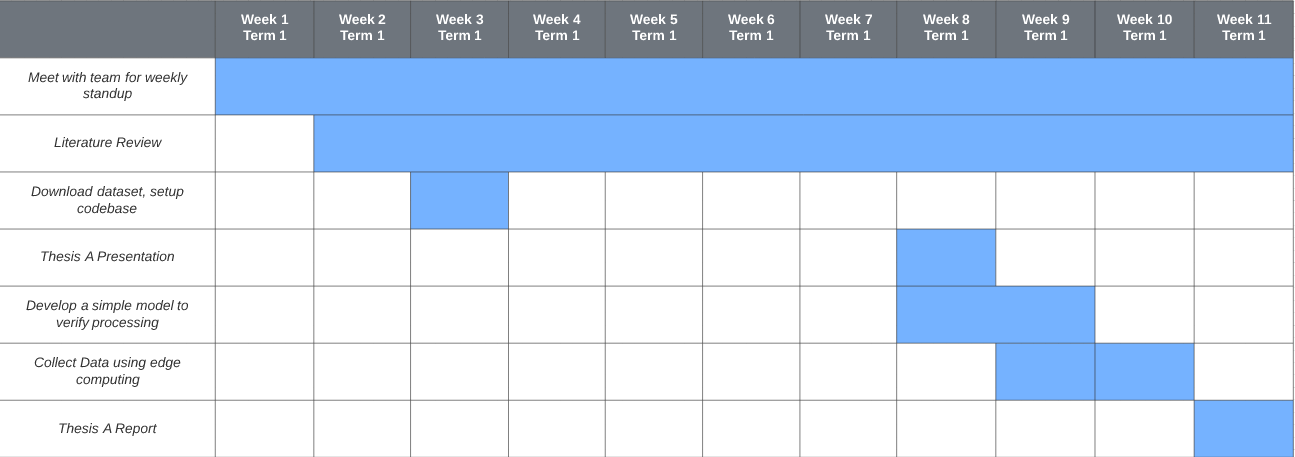
\includegraphics[width=400px, keepaspectratio]{gant1.png}
    \vspace{1ex}%
    \caption{Gantt chart for thesis A.}
    \label{fig:my_label}
\end{figure}

\begin{figure}[H]
    \centering
    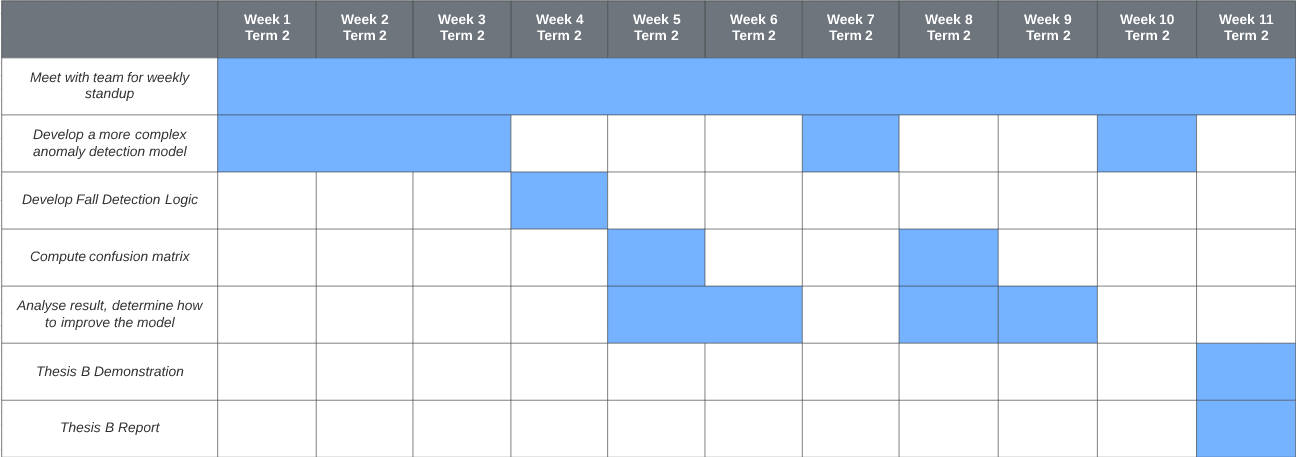
\includegraphics[width=400px, keepaspectratio]{gant2.png}
    \vspace{1ex}%
    \caption{Gantt chart for thesis B.}
    \label{fig:my_label}
\end{figure}

\begin{figure}[H]
    \centering
    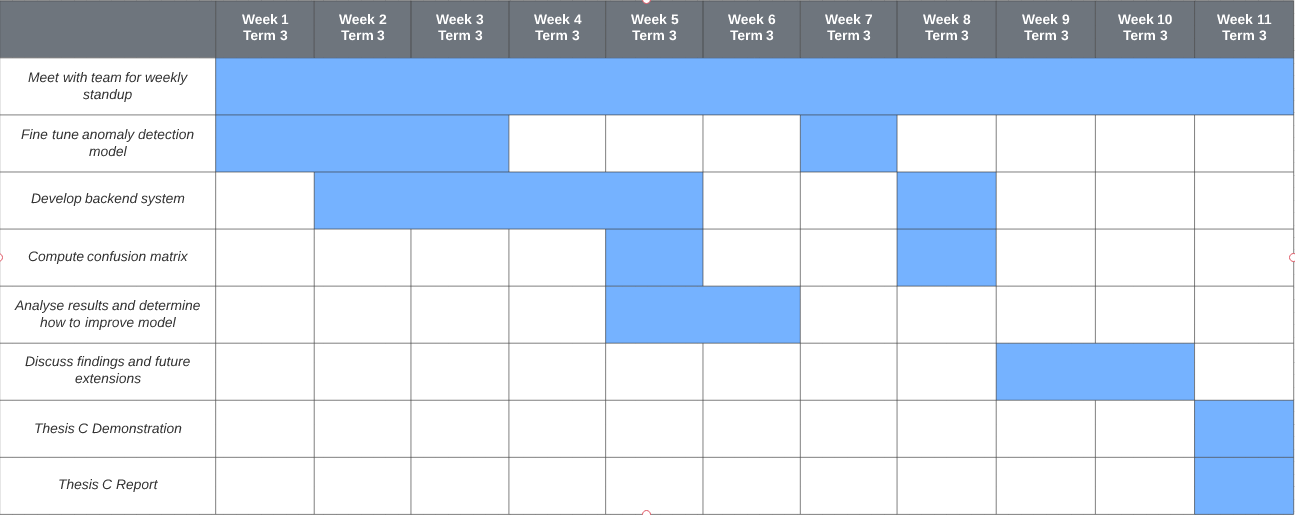
\includegraphics[width=400px, keepaspectratio]{gant3.png}
    \vspace{1ex}%
    \caption{Gantt chart for thesis C.}
    \label{fig:my_label}
\end{figure}